%%%%%%%%%%%%%%%%%%%%%%%%%%%%%%%%%%%%%%%%%
% Wenneker Assignment
% LaTeX Template
% Version 2.0 (12/1/2019)
%
% This template originates from:
% http://www.LaTeXTemplates.com
%
% Authors:
% Vel (vel@LaTeXTemplates.com)
% Frits Wenneker
%
% License:
% CC BY-NC-SA 3.0 (http://creativecommons.org/licenses/by-nc-sa/3.0/)
% 
%%%%%%%%%%%%%%%%%%%%%%%%%%%%%%%%%%%%%%%%%

%----------------------------------------------------------------------------------------
%	PACKAGES AND OTHER DOCUMENT CONFIGURATIONS
%----------------------------------------------------------------------------------------

\documentclass[11pt]{scrartcl} % Font size

%%%%%%%%%%%%%%%%%%%%%%%%%%%%%%%%%%%%%%%%%
% Wenneker Assignment
% Structure Specification File
% Version 2.0 (12/1/2019)
%
% This template originates from:
% http://www.LaTeXTemplates.com
%
% Authors:
% Vel (vel@LaTeXTemplates.com)
% Frits Wenneker
%
% License:
% CC BY-NC-SA 3.0 (http://creativecommons.org/licenses/by-nc-sa/3.0/)
% 
%%%%%%%%%%%%%%%%%%%%%%%%%%%%%%%%%%%%%%%%%

%----------------------------------------------------------------------------------------
%	PACKAGES AND OTHER DOCUMENT CONFIGURATIONS
%----------------------------------------------------------------------------------------

\usepackage{amsmath, amsfonts, amsthm} % Math packages

\usepackage{listings} % Code listings, with syntax highlighting

\usepackage[main = greek, english]{babel} % English language hyphenation

\usepackage{graphicx} % Required for inserting images
\graphicspath{{Figures/}{./}} % Specifies where to look for included images (trailing slash required)

\usepackage{booktabs} % Required for better horizontal rules in tables

\usepackage{dirtytalk} % Required for quoting.

\usepackage{float} % Added for hard placement of images.

\usepackage[dvipsnames]{xcolor} % Added for extra colors.

\usepackage{tikz} % For colored boxes and more.

\numberwithin{equation}{section} % Number equations within sections (i.e. 1.1, 1.2, 2.1, 2.2 instead of 1, 2, 3, 4)
\numberwithin{figure}{section} % Number figures within sections (i.e. 1.1, 1.2, 2.1, 2.2 instead of 1, 2, 3, 4)
\numberwithin{table}{section} % Number tables within sections (i.e. 1.1, 1.2, 2.1, 2.2 instead of 1, 2, 3, 4)

\usepackage{enumitem} % Required for list customisation
\setlist{noitemsep} % No spacing between list items

%----------------------------------------------------------------------------------------
%	DOCUMENT MARGINS
%----------------------------------------------------------------------------------------

\usepackage{geometry} % Required for adjusting page dimensions and margins

\geometry{
	paper=a4paper, % Paper size, change to letterpaper for US letter size
	top=2.5cm, % Top margin
	bottom=3cm, % Bottom margin
	left=3cm, % Left margin
	right=3cm, % Right margin
	headheight=0.75cm, % Header height
	footskip=1.5cm, % Space from the bottom margin to the baseline of the footer
	headsep=0.75cm, % Space from the top margin to the baseline of the header
	%showframe, % Uncomment to show how the type block is set on the page
}

%----------------------------------------------------------------------------------------
%	FONTS
%----------------------------------------------------------------------------------------

\usepackage[utf8]{inputenc} % Required for inputting international characters
\usepackage[T1]{fontenc} % Use 8-bit encoding

%----------------------------------------------------------------------------------------
%	SECTION TITLES
%----------------------------------------------------------------------------------------

\usepackage{sectsty} % Allows customising section commands

\sectionfont{\vspace{6pt}\centering\normalfont\scshape} % \section{} styling
\subsectionfont{\normalfont\bfseries} % \subsection{} styling
\subsubsectionfont{\normalfont\itshape} % \subsubsection{} styling
\paragraphfont{\normalfont\scshape} % \paragraph{} styling

%----------------------------------------------------------------------------------------
%	HEADERS AND FOOTERS
%----------------------------------------------------------------------------------------

\usepackage{scrlayer-scrpage} % Required for customising headers and footers

\ohead*{} % Right header
\ihead*{} % Left header
\chead*{} % Centre header

\ofoot*{} % Right footer
\ifoot*{} % Left footer
\cfoot*{\pagemark} % Centre footer

\newcommand{\img}[1]
{
    \begin{center}
        \fcolorbox{black}{white}{\includegraphics[height=10em]{#1}}
    \end{center}

}

% Helper Macros

\newcommand{\en}[1]{\foreignlanguage{english}{#1}}
\newcommand{\src}[1]{{\ttfamily\en{#1}}}


% Extra Formatting

\setlength{\parindent}{0em}
\setlength{\parskip}{1em}
 % Include the file specifying the document structure and custom commands

\usepackage{subcaption}
\usepackage{amsmath}
\usepackage{listings}
\usepackage{pgfplots}

\pgfplotsset{compat = newest}
\lstset{language=C++}
\lstset{% general command to set parameter(s)
basicstyle=\small\ttfamily, % print whole listing small
keywordstyle=\color{black}\bfseries\underbar,
% underlined bold black keywords
identifierstyle=, % nothing happens
stringstyle=\ttfamily, % typewriter type for strings
showstringspaces=false} % no special string spaces
\lstset{numbers=left, numberstyle=\ttfamily}
% \lstset{backgroundcolor=\color{Blue}}

%----------------------------------------------------------------------------------------
%	TITLE SECTION
%----------------------------------------------------------------------------------------

\title{	
	\normalfont\normalsize
	\textsc{Πανεπιστήμιο Πατρών, Τμήμα Ηλεκτρολόγων Μηχανικών και Τεχνολογίας Υπολογιστών}\\ % Your university, school and/or department name(s)
	\vspace{25pt} % Whitespace
	\rule{\linewidth}{0.5pt}\\ % Thin top horizontal rule
	\vspace{20pt} % Whitespace
	{\Large Εργασία: \en{Pokemon}}\\ % The assignment title
	\vspace{12pt} % Whitespace
	\rule{\linewidth}{2pt}\\ % Thick bottom horizontal rule
	\vspace{12pt} % Whitespace
}

\author{\LARGE Ευάγγελος Λάμπρου \\ \en{UP1066519}} % Your name

\date{} % Today's date (\today) or a custom date

\begin{document}

\maketitle 

\tableofcontents

\newpage

\section{Εισαγωγή}

\section{Ερωτήματα Εργασίας}

\subsection{Μέρος Α}

\subsubsection{Δημιουργία σκηνής κόσμου.}

Ο κόσμος τη εργασίας είναι ένα απλό τοπίο αποτελούμενο από δέντρα και βράχους. Σε κάθε εκτέλεση της εφαρμογής
δημιουργείται ένα νέο τυχαίο τοπίο, με τα αντικείμενα της σκηνής να τοποθετούνται σε τυχαίες θέσεις. 

Για το \en{skybox}, ακολούθησαμε την τεχνική όπου τοποθετούμε στον ορίζοντα το μοντέλο ενός κύβου το οποίο 
στις πλευρές του έχει σαν \en{texture} την κάθε μία από τις όψεις του ουρανού.

% Skybox picture

Δώσαμε ακόμα στον κόσμο έναν κύκλο ημέρας-νύκτας, αλλάζοντα το χρώμα του \en{skybox} σταδιaκά. Συγκεκριμένα, 
εφαρμόζουμε \en{interpolation} \say{ανταλλάζοντας} τα \en{red} και \en{blue} \en{channels} με βάση μία ημιτονοειδή συνάρτηση.

% Two skybox pictures: night and day

\begin{equation}
    color = mix(color_{texture}.bgr, color_{texture}.rgb, \frac{sin(time) + 1}{2})
\end{equation}

\begin{figure}[H]
    \begin{center}
    \begin{tikzpicture}
        \begin{axis}[xmin=0, xmax=10*pi, ymin=-1, ymax=1]
            \addplot[
                domain = 0:10*pi,
                samples = 200,
                smooth,
                thick,
            ] {sin(30*x)};
        \end{axis}
    \end{tikzpicture}
        \caption{Η συνάρτηση ημιτόνου.}
        \end{center}
\end{figure}

Ως πηγή φωτισμού θεωρούμε τον ήλιο. Συνεπώς ερφαρμόζουμε την τεχνική \en{directional lighting} όπου 
κάθε \en{vertex} των αντικειμένων της σκηνής μας φωτίζονται από την ίδια κατεύθυνση ανεξαρτήτως της θέσης τους.
Πρακτικά θεωρούμε πως η πηγή φωτός απέχει μία άπειρη απόσταση από τα υπόλοιπα αντικείμενα της σκηνής μας.
Έτσι, τοποθετήσαμε προσεγγιστικά τον ήλιο σε ένα \say{ψηλό} σημείο. 

% Sun pictures

\subsubsection{Μέθοδος σκίασης}

Η σκίαση της σκηνής αποτέλεσε ένα από τα δυσκολότερα μέρη της εργασίας. Ωστόσο, το τελικό αποτέλεσμα 
είναι ικανοποιητικό. 

Η μέθδος που χρησιμοποιήσαμε είναι αυτή του \en{shadow mapping}. Ζωγραφίζουμε την σκηνή από την πλευρά 
της πηγής φωτός (του ήλιου) σε ένα \en{texture} στο οποίο αποτυπώνεται η απόσταση του κάθε αντικειμένου 
από το φως. Έτσι, μπορούμε να συμπεράνουμε εάν ένα σημείο σκιάζεται. 

Για να δωθεί περαιτέρω η αίσθηση για το πέρασμα του χρόνου, έχουμε την φωτεινή πηγή να κινείται 
γύρω από τη σκηνή για να προσομοιώσει την κίνηση του ήλιου. 
Για αυτό το λόγο στη σκηνή μας περιοριζόμαστε σε \en{dynamic shadows}.

% Picture with shadows

\subsubsection{Περιήγηση στη σκηνή και φυσική αλληλεπίδραση}

Για την περιήγηση του χρήστη στη σκηνή, δημιοργήσαμε μία οντότητα κάμερας η οποία είναι υπεύθυνση 
για τον υπολογισμό των \en{view} και \en{projection} πινάκων με βάση μία δεδομένη θέση και κατεύθυνση όρασης.

Για να προσθέσουμε φυσικές ιδιότητες στα αντικείμενα της σκηνής, τους προσθέσαμε ιδιότητες στερεού σώματος (\en{rigid body}).
Συγκεκριμένα, σε κάθε καρέ της εφαρμογής υπολογίζουμε τη νέα θέση και ταχύτητα του κάθε αντικειμένου με βάση το διάνυσμα κατάστασής 
του. Αυτό το διάνυσμα περιέχει πληροφορίες όσων αφορά την τωρινή του θέση, ορμή, γωνιακή ταχύτητα, στροφορμή και περιστροφή.

Για να υπολογίσουμε την κάθε επόμενη κατάσταση χρησιμοποιούμε την μέθοδο αριθμητικής ολοκλήρωσης \en{Runge-Kuta} 4ης τάξης.


\begin{figure}[H]
\begin{gather}
    s(t)
     =
  \begin{bmatrix}
      x(t) \\
      R(t) \\ 
      P(t) \\
      L(t) \\
   \end{bmatrix}
\end{gather}
    \caption{Το διάνυσμα κατάστασης.}
\end{figure}

Έτσι, έχουμε αντικείμενα τα οποία μπορούν να υπακούν στο νόμο της βαρύτητας και στα οποία μπορούμε να 
εφαρμόζουμε αυθαίρετες δυνάμεις.

Για να υπάρχει, ωστόσο, αλληλεπίδραση μεταξύ των αντικειμένων ορίσαμε ένα σύστημα ανίχνευσης συγκρούσεων (\en{collision detection}). 
Σε κάθε αντικείμενο της σκηνής προσθέσαμε ένα \en{AABB (axis-aligned bounding box)}. Δηλαδή, έναν κύβο του οποίου 
οι οκτώ (8) κορυφές βρίσκονται στα ακραία \en{vertices} του αντικειμένου. 
Σε περίπτωση όπου στο αντικείμενο εφαρμοστούν \en{transformations}, αυτές επηρεάζουν και το αντίστοιχό του \en{AABB}.
Τελικά, ο έλεγχος συγκρούσεων γίνεται απλά μία υπόθεση σύγκρισης των συντεταγμένων των κορυφών μεταξύ δύο \en{AABBs}.

\begin{figure}[H]
    \begin{center}
\begin{tikzpicture}
    % https://tex.stackexchange.com/questions/285578/how-to-draw-parallelepiped-and-cube-with-latex/288101#288101
    \pgfmathsetmacro{\cubex}{2}
    \pgfmathsetmacro{\cubey}{1}
    \pgfmathsetmacro{\cubez}{1}
    \draw[red,fill=white] (0,0,0) -- ++(-\cubex,0,0) -- ++(0,-\cubey,0) -- ++(\cubex,0,0) -- cycle;
    \draw[red,fill=white] (0,0,0) -- ++(0,0,-\cubez) -- ++(0,-\cubey,0) -- ++(0,0,\cubez) -- cycle;
    \draw[red,fill=white] (0,0,0) -- ++(-\cubex,0,0) -- ++(0,0,-\cubez) -- ++(\cubex,0,0) -- cycle;

    \pgfmathsetmacro{\cubex}{2}
    \pgfmathsetmacro{\cubey}{1}
    \pgfmathsetmacro{\cubez}{1}
    \draw[red] (1,0.5,0) -- ++(-\cubex,0,0) -- ++(0,-\cubey,0) -- ++(\cubex,0,0) -- cycle;
    \draw[red] (1,0.5,0) -- ++(0,0,-\cubez) -- ++(0,-\cubey,0) -- ++(0,0,\cubez) -- cycle;
    \draw[red] (1,0.5,0) -- ++(-\cubex,0,0) -- ++(0,0,-\cubez) -- ++(\cubex,0,0) -- cycle;
\end{tikzpicture}
    \end{center}
    \caption{Παράδειγμα ελέγχου σύγκρουσης με δύο \en{AABBs}.}
\end{figure}

Με το πάτημα του πλήκτρου \en{T} ο χαρακτήρας μας εκτοξεύει μία σφαίρα προς την κατεύθυνση που κοιτάει. Αυτή η σφαίρα
αλληλεπιδρά με τις οντότητες του κόσμου της σκηνής αλλά και με άλλες σφαίρες. Ο μαθηματικός τύπος
ο οποίος θα μας δίνει τη νέα ταχύτητα της σφαίρας μετά από μία σύγκρουση πέρασε από διάφορες αλλαγές. 

Μία επιλογή είναι ο προσεγγιστικός τύπος της ελαστικής κρούσης:

\begin{equation}
    % auto v = velocity - 2.0f * glm::dot(velocity, collision_direction) * collision_direction;
    \vec{v}^\prime = \vec{v} - 2 \cdot ( \vec{v} \cdot \vec{n} ) \cdot \vec{n}
\end{equation}

Ο οποίος δίνει ρεαλιστικά αποτελέσματα αλλά απαιτεί διορθώσεις λόγω του τρόπου με τον οποίο υπολογίζουμε το διάνυσμα 
σύγκρουσης $\vec{n}$. 

Μία άλλη επιλογή ήταν ο απλοϊκός τύπος 

\begin{equation}
    \vec{v}^\prime = -\vec{v}
\end{equation}

Ο οποίος κάνει της συγκρούσεις των σφαιρών με το περιβάλλον να μοιάζουν με σκηνή \say{καρτούν}. Αυτό, φυσικά 
δεν είναι κάτι ανεπιθύμητο, αλλά έγινε προσπάθεια για πιο ρεαλιστικές συγκρούσεις.

Τέλος, δώσαμε και στον παίκτη φυσικές ιδιότητες, δίνοντάς του ιδιότητες ενός \en{rigid body}. 
Ο χρήστης μπορεί να ανεβαίνει πάνω στα αντικείμενα της σκηνής, να πηδάει και να πετάει.

% Picture of balls bouncing realistically 
% Picture of balls bouncing comically

\subsection{Μέρος Β}

\subsubsection{Εμφάνιση τέρατος}

Εφόσων μία σφαίρα αναπηδήσει τρεις φορές στο έδαφος, εμφανίζεται στη σκηνή ένα τέρας στη θέση της. Το εφέ που 
χρησιμοποιήσαμε είναι ένα εφέ καπνού. Ζωγραφίζουμε με το σύστημα σωματιδίων (\en{particle system}) 
έναν μεγάλο αριθμό από γκρίζους κύβους οι οποίοι κινούνται προς τα πάνω. 
Με το πέρασμα του χρόνου, μέσα από τον \en{shader} ο οποίος χειρίζεται αυτά τα \say{σωματίδια} τα μεγενθύνουμε
και μειώνουμε την τιμή του \en{alpha}, κάνοντάς τα μετά από πέντε (5) δευτερόλεπτα διάφανα. 

Υπάρχει ένας εύκολος τρόπος να μεγνθύνουμε ομογενώς ένα αντικείμενο μέσα από τον \en{vertex shader} όπως φαίνεται 
στον κώδικα (\ref{ezbigger_vert}).

\begin{minipage}{\textwidth}
\selectlanguage{english}
\begin{lstlisting}[caption=\textgreek{Μεγέθυνση αντικειμένου από τον} vertex shader, label=ezbigger_vert]
// scale the object by a factor of c
vec4 pos = vec4(vertex_position * c, 1.0);
gl_Position = mvp * pos;
\end{lstlisting}
\end{minipage}
\selectlanguage{greek}
Ακόμα, για λόγους απόδοσης περιοριστήκαμε σε απλά μοντέλα για το κάθε σωματίδιο (κύβοι και σφαίρες) 
ώστε να έχουμε χαμηλό αριθμό από \en{vertices}. Εφαρμόσαμε επίσης την τεχνική του \en{instancing}
κατά το οποίο ζωγραφίζουμε στην οθόνη πολλά αντικείμενα τα οποία μοιράζονται το ίδιο \en{VAO}
σε ένα (1) μόνο  \en{draw call} στην κάρτα γραφικών.

% pictures of the smoke
 
Για τα μοντέλα των τεράτων χρησιμοποιήσαμε αρχεία \en{objs} από διάφορους ιστιότοπους. 

% pictures of the monsters

\subsubsection{Παγίδευση τέρατος}

Πατώντας το πλήκτρο \en{C}, ο χρήστης μπορεί να επιλέξει μεταξύ των δύο ειδών 
σφαίρας οι οποίες είναι:
\begin{enumerate}
    \item Μπάλες που θα εμφανίσουν ένα τέρας όταν συγκρουστούν με το έδαφος.
    \item Μπάλες που θα παγιδεύσουν ένα τέρας όταν συγκρουστούν με αυτό.
\end{enumerate}

Αν ο χρήστης επιλέξει το δεύτερο είδος σφαίρας μπορεί να σημαδεύσει σε ένα τέρας και 
έτσι να το παγιδεύσει. Όταν το παγιδεύει έχουμε ένα απλό εφέ αστεριών. 

% picture of stars when capturing monster

\subsubsection{Επίθεση τέρατος}

Συνολικά έχουμε τρία (3) διαφορετικά τέρατα. Ένα τέρας φωτιάς, ένα τέρας τοξικής ομίχλης και ένα τέρος ηλκετρισμού.

% Pictures of all three monsters

Το καθένα έχει μία διαφορετική επίθεση.

\subsection{\en{Bonus}}

\subsubsection{Εξέλιξη τέρατος}

Η υλοποίηση μιας εξέλιξης τέρατος έγινε δημιουργώντας αρχικά 

\begin{figure}[H]
	\begin{center}
		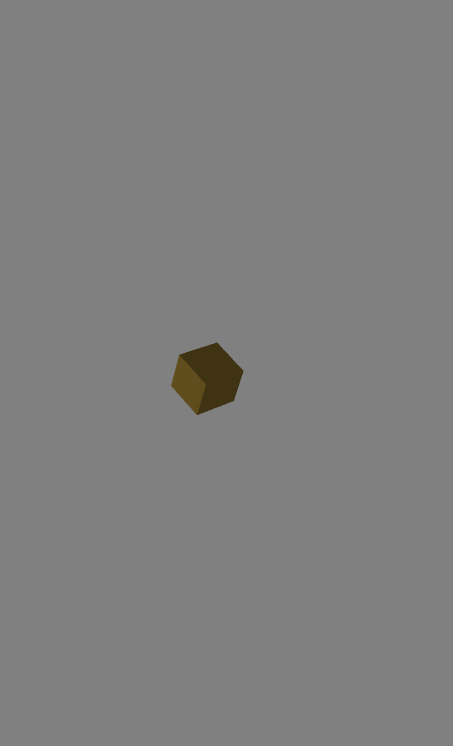
\includegraphics[height=.5\textheight]{./assets/cube.png}
	\end{center}
	\caption{Ο κύβος να περιστρέφεται}
\end{figure}

\end{document}
